质点是对运动物体的简化模型，它的运动学性质集中体现为它作为“点”的一面，可以用质
点的位置随时间的变化关系给出，在运动学的学习中已经广泛讨论了质点和由多个质点构
成的质点系统的运动。与此同时，质点还具有质量。质量是物体的一个基本属性；对于均匀的物质
来说，它的质量由物质的密度和体积的乘积共同决定；如果一个物体由多个部分组成，则其质量
为组成它的各部分质量之和。

具有相同速度但质量不同的质点，表现出的运动性质并不相同。为了体现这种不同，定义一个
新的物理量——动量。它是一个矢量，定义为质点的质量和速度的乘积，方向与质点的速度方向相同：
\begin{equation}
  \vec p=m\vec v.
\end{equation}
在相同外力作用下，质量越大的物体运动状态的变化越不明显；反之，力作用于质量较小的物体
时，则会引起较大的速度变化。

在大量经验和实验的基础上，英国物理学家牛顿给出了支配物体运动的三大定律：
\begin{description}[style=nextline,leftmargin=2em,labelindent=0pt]
  \item[第一定律]不受外力作用的物体必将保持静止或做匀速直线运动。
  \item[第二定律]物体的动量随时间的变化率等于所受的合外力；质量不变时，加速度由合外力决定。
  \item[第三定律]任意两个物体之间的相互作用力大小相等、方向相反，并且在一条直线上。
\end{description}
牛顿的三个运动定律是动力学的基础，相当精确地给出了宏观物体的运动规律。作为最基本的运动
定律，有必要深入讨论它们适用的条件，以及它们对自然现象的解释。

\subsection{第一定律：惯性}

牛顿第一定律又被称为惯性定律，指出了物体在不受外力作用时“应有”的运动状态，即运动学
中最简单的运动——匀速直线运动。惯性是任何物体所固有的属性，它使物体有保持原有运动状态，
也就是保持速度的趋势。惯性本身也可以度量，其大小的量度正是物体本身的质量。质量越大，物体
的惯性越大；在相同力的作用下，其运动状态的改变反而越小。

在运动学中可以在任意参考系中建立合适的坐标系来描写物体的运动，但在动力学中，牛顿定律并不
能适用于所有参考系，而只能适用于一类特殊的参考系，称为惯性参考系或惯性系。只有在惯性系中，
不受力物体的运动才是匀速直线运动。

惯性系的选取并不唯一。当参考系 $S$ 是惯性系时，所有相对于 $S$ 做匀速直线运动的参考系都是
惯性系。同一个不受力质点在不同惯性系中均做匀速直线运动，只不过运动速度不同。而相对于
$S$ 做加速运动的参考系则不是惯性系，牛顿定律若要在其中使用，必须加以改写。

关于是否存在真正的惯性参考系、在哪里能够找到惯性系，长期以来一直是极具争论的话题。绝大多数
力学现象都以地球表面为参考系来描写；实践表明，在地表参考系中应用牛顿定律，已经能够以相当高的
精度描述日常物体的运动。但是，对运动范围较广、速度较快或观测精度较高的过程，地表就不能再当作
严格的惯性系。地球不但自转，还绕太阳公转，这些转动都意味着地表参考系具有加速度。

以太阳为参考系时，牛顿定律能够在更高的精度上成立；然而天文观测又表明，太阳带着太阳系中的天体
以很高的速度绕银河系中心运动，虽然它的加速度很小，却也不是严格意义上的惯性参考系。关于惯性系
的争论始终存在，爱因斯坦的相对论给出了部分答案，同时又面临宇宙学问题的进一步检验。在实践中，
如果没有特别说明，描写地球上速度不高、范围不大、持续时间不长的物理过程时，通常近似取地表为
惯性系；相对于地面做加速运动的参考系则是非惯性系。

\noindent\textbf{【思考】}你能够发挥想象力，或通过已知的物理知识给出一个惯性参考系吗？

\begin{thinkanswer}
严格惯性系是一种理想化概念，实际中只能根据问题精度选择足够好的近似。在普通地面力学问题中，
地面参考系就是实用的近似惯性系；研究行星运动时，可选以太阳系质心为原点、坐标轴指向遥远天体的
参考系。判断关键不在于某个参考系的名字，而在于其非惯性效应是否小到可在当前精度下忽略。
\end{thinkanswer}

\subsection{第二定律：加速}

第一定律指出，不受力的物体在惯性系中运动速度不会发生变化；第二定律进一步告诉我们，
当物体受到力的作用时，其运动状态如何发生变化。利用动量，第二定律可写成
\begin{equation}
  \vec F=\frac{\dd\vec p}{\dd t}.
\end{equation}
在牛顿力学的常见问题中，物体的质量在运动过程中保持不变，根据动量的定义，上式化为更常用的形式
\begin{equation}
  \vec F=m\vec a.
\end{equation}
即质量与加速度的乘积等于物体所受的合外力，加速度的方向与合外力方向相同。使用牛顿第二定律
时需要注意：
\begin{itemize}
  \item 和第一定律一样，牛顿第二定律也只在惯性系中按上述形式成立。在非惯性系中，必须引入惯性力后才能使用类似形式。
  \item 经典形式适用于宏观、低速物体。接近光速的运动和微观粒子的运动需要其它物理理论。
  \item 当一个物体同时受到多个力时，决定加速度的 $\vec F$ 是所有外力的矢量和。
\end{itemize}

\noindent\textbf{【思考】}牛顿第一定律是否仅仅是第二定律在 $\vec F=0$ 时的特例？

\begin{thinkanswer}
不是简单的重复。如果已经预先确定了惯性系，由 $\vec F=m\vec a$ 确实可在 $\vec F=0$ 时得到 $\vec a=0$。
但第一定律同时给出了惯性系的判别标准，也说明物体保持匀速直线运动并不需要力来维持。第二定律要有明确物理意义，
已经隐含了“在惯性系中”这一前提；这个前提正是第一定律所确立的。
\end{thinkanswer}

第二定律有两类典型应用：一类是通过观察到的运动确定物体所受外力的性质；另一类是在已知所有外力
时预测物体未来的运动。例如：

研究物体运动的早期工作，常常从观察具体运动入手，再利用第二定律推测外力的大小、方向与物体性质、
外界条件之间的关系。运动学中出现的各种运动形式，从动力学角度看，都是力改变运动状态的结果；质量
为 $m$ 的物体若做某种已知运动，它在每一时刻所受合外力必为 $m$ 与该时刻加速度的乘积。通过分析
运动过程，便可反过来认识多种相互作用力。
\begin{itemize}
  \item 地表附近抛出的物体均做抛体运动，加速度大小为 $g$、方向竖直向下，因此质量为 $m$ 的物体在飞行过程中始终受到重力
  \begin{equation}
    F=mg.
  \end{equation}
  重力指向地面，其作用点可等效取在物体的重心。
  \item 做匀速圆周运动的质点具有指向圆心的加速度。质量为 $m$ 的质点以速率 $v$ 做半径为 $R$ 的圆周运动时，合外力必须指向圆心，大小为
  \begin{equation}
    F=m\frac{v^2}{R}.
  \end{equation}
  这个时刻指向圆心的合力通常称为向心力；若没有这样的合力，质点将依照第一定律沿直线运动。
  \item 太阳系各行星的运动满足开普勒三定律。通过分析行星运动可知，行星所受的力时刻指向太阳；在这些结论基础上，牛顿进一步作出大胆概括，得到万有引力定律。任意两个物体之间都有指向对方的引力，其大小为
  \begin{equation}
    F=G\frac{m_1m_2}{r^2}.
  \end{equation}
  万有引力是牛顿力学最重要的成果之一，后面将专门讨论它的性质和应用。
  \item 当物体的运动受到约束时会受到约束力。与重力、弹簧弹力等不同，约束力的大小和方向往往不能在一开始就决定，而要由物体所受的其它力以及运动状态共同确定。平面的弹力、连杆内的弹力、绳子的拉力都是典型的约束力；相当一部分问题的复杂性，正来自需要在运动的不同时刻确定这些约束力。
  \item 自然界还广泛存在各种阻力，它们会降低机械效率，也会增加预测运动的难度。当两物体接触且存在相对运动或相对运动趋势时，会出现滑动摩擦力或静摩擦力。常见的滑动摩擦力通常与接触面压力 $N$ 成正比，方向与相对运动方向相反：
  \begin{equation}
    f=\mu N.
  \end{equation}
  其中比例系数 $\mu$ 是摩擦因数，与接触物体的性质有关。水中或空气中运动的物体也会受到阻力；流体阻力由流体性质、运动物体的形状和速度共同决定，通常难以简单定量描述，后面将在若干理想化条件下讨论。
\end{itemize}

\subsection{从物理对象到运动方程}

牛顿定律的应用不是把若干力机械地写进公式，而是先说明研究对象、参考系和作用过程。
把一个物体单独取出时，凡是来自系统边界以外的相互作用都要画在受力图上；物体内部各部分
之间的作用不应重复计入。重力由质量和重力场决定，弹簧弹力由形变量决定，支持力、绳张力
和静摩擦力却通常要与运动约束一起求出。因此受力图上可以先标未知量，但不能凭经验预先
认定它们的大小，更不能把“运动方向”误当成“合力方向”。

选定惯性系后，质点的运动方程为
\begin{equation}
 \frac{\dd\vec p}{\dd t}=\sum_i\vec F_i,
 \qquad\text{质量不变时为}\qquad
 m\ddot{\vec r}=\sum_i\vec F_i.
\end{equation}
这是一个矢量方程。若在直角坐标系中使用，就应在每个方向分别投影；若轨迹弯曲，沿切向与
法向分解往往更直接：切向分量改变速率，法向分量改变速度方向。得到加速度以后，还必须结合
初始位置和初速度积分，运动才被唯一确定。由此可见，同一受力方程配上不同初始条件，可以
描述完全不同的运动。

约束把不同物体的运动联系起来。不可伸长轻绳给出绳长不变；对于方向不转动的平面接触，
保持接触意味着物体与平面沿固定法向的加速度相同；纯滚动给出接触点相对速度为零。
曲面接触则不能直接照搬“法向加速度相同”。例如质点沿固定圆轨道运动时，
由 $\vec r\cdot\vec r=R^2$ 先求导得 $\vec r\cdot\vec v=0$，再求导得
$\vec r\cdot\vec a=-v^2$，因此即使轨道静止，质点仍有大小 $v^2/R$ 的向心加速度。
一般约束须先写几何关系，再对时间求导，不能遗漏曲率或转动带来的项。
可靠的列式顺序是：分别画受力图，选取便于投影的方向，
为每个独立物体列动力学方程，再用几何或运动学约束把未知量闭合。方程数量不足时，往往不是
“少列了一条牛顿定律”，而是遗漏了一个约束关系。

牛顿第三定律说明相互作用总是成对出现：$\vec F_{A\to B}=-\vec F_{B\to A}$。这两个力作用在
不同物体上，所以不能在单个物体的受力图中相互抵消；只有把 $A,B$ 作为一个整体研究时，它们
才成为内力并在系统合力中消去。第三定律还要求同时、共线，并与两个物体是否静止无关。
处理多物体问题时，先整体求加速度、再隔离局部求张力或支持力，正是利用了这一结构。


\begin{origexamplebox}{例 2.1}
一个质量为 $m$，沿平面上 $x$ 轴运动质点的位置随时间的关系为
\[
  x(t)=A\cos\omega t,
\]
求它所受到外力随位置的关系。
\end{origexamplebox}

\begin{xesolution}
对位置函数连续求两次导数：
\[
  v_x=\frac{\dd x}{\dd t}=-A\omega\sin\omega t,
  \qquad
  a_x=\frac{\dd^2x}{\dd t^2}=-A\omega^2\cos\omega t=-\omega^2x.
\]
因此外力与位置的关系为
\[
  \boxed{F_x(x)=-m\omega^2x}.
\]
负号的几何意义如解图所示：
\soldiagTwoOne
当 $x>0$ 时力向左，当 $x<0$ 时力向右；合力始终指向平衡位置 $x=0$。
\end{xesolution}

\begin{origexamplebox}{例 2.2}
在一固定平面上，一个质点的运动由方程
\[
  x(t)=A\cos\omega t,
  \qquad
  y(t)=A\sin\omega t
\]
给出，其中 $A>0$、$\omega>0$，质点质量为 $m$。求它在运动过程中的合外力。
\end{origexamplebox}

\begin{xesolution}
对两个坐标分别求二阶导数：
\[
  \ddot x=-\omega^2x,
  \qquad
  \ddot y=-\omega^2y.
\]
故
\[
  \boxed{\vec F=-m\omega^2(x\,\hat{\boldsymbol i}+y\,\hat{\boldsymbol j})
  =-m\omega^2\vec r}.
\]
又因为 $x^2+y^2=A^2$，质点做半径为 $A$ 的匀速圆周运动。速度为
\[
 \vec v=A\omega(-\sin\omega t\,\hat{\boldsymbol i}
 +\cos\omega t\,\hat{\boldsymbol j}).
\]
从 $t=0$ 的 $(A,0)$ 点出发时速度向上，故运动方向是逆时针。图中 $P$ 位于第一象限，
其速度沿切线指向左上，而合力沿半径指向 $O$：
\soldiagTwoTwo
合力时刻指向圆心，大小为
\[
  \boxed{F=m\omega^2A}.
\]
\end{xesolution}

\begin{origexamplebox}{例 2.3}
质量为 $m$ 的物体受何种合外力，可以使其按下列方程运动？
\[
  x(t)=A\cos\omega t,
  \qquad y(t)=A\sin\omega t,
  \qquad z(t)=q(t)
\]
其中 $A>0$、$\omega>0$，$q(t)$ 是给定的二阶可导位置函数。另讨论 $q(t)=ut$、$u$ 为常量的情形。
\end{origexamplebox}

\begin{xesolution}
三个方向的加速度为
\[
  \ddot x=-A\omega^2\cos\omega t,
  \qquad
  \ddot y=-A\omega^2\sin\omega t,
  \qquad
  \ddot z=q''(t).
\]
因此所需合外力为
\[
  \boxed{\vec F(t)=
  -m\omega^2\bigl[x(t)\hat{\boldsymbol i}+y(t)\hat{\boldsymbol j}\bigr]
  +mq''(t)\hat{\boldsymbol k}}.
\]
水平合力指向 $z$ 轴，竖直合力由 $q''(t)$ 决定；不能仅凭水平投影为圆便断定合力没有竖直分量。
若 $q(t)=ut$，则 $\dot z=u$、$\ddot z=0$，轨迹为等螺距螺旋线：$u>0$ 时上升，
$u<0$ 时下降，$u=0$ 时退化为圆。图取 $u>0$，$H$ 是与 $P$ 等高的轴上点，
$PH$ 位于水平面内；$P_0$ 是 $P$ 在 $xy$ 平面上的投影。
\Needspace{12\baselineskip}
\soldiagTwoThree
在这一特例中合外力没有竖直分量，大小恒为 $m\omega^2A$。每转一周历时 $2\pi/\omega$，
竖直位移为 $2\pi u/\omega$。一般情况下，合力大小则为
$m\sqrt{\omega^4A^2+[q''(t)]^2}$；两项的量纲均为加速度的平方。
\end{xesolution}

\begin{origexamplebox}{例 2.4}
在一个研究质点在特定介质中运动所受阻力的实验中发现，一个质量为 $m$、初速度为 $v_0$
的质点在阻力作用下减速，且速度随它在介质中前进的距离的变化关系为
\[
  v(x)=v_0-\alpha x,\qquad v_0>0,\quad\alpha>0.
\]
探讨它所受阻力的形式。
\end{origexamplebox}

\begin{xesolution}
在质点仍沿 $+x$ 方向运动时，利用链式求导
\[
  a=\frac{\dd v}{\dd t}
  =\frac{\dd v}{\dd x}\frac{\dd x}{\dd t}
  =(-\alpha)v.
\]
所以
\[
  \boxed{F_x=-m\alpha v=-m\alpha(v_0-\alpha x)}.
\]
力与运动方向的关系如解图所示：
\soldiagTwoFour
因此阻力的大小与瞬时速度成正比，方向与速度相反。左图是速度与位置的函数图，右图才是在
真实空间中对质点作出的受力示意，二者不能混为同一幅位置图。
进一步用初值 $v(0)=v_0$ 解运动方程：
\[
 \frac{\dd v}{\dd t}=-\alpha v,
 \qquad\int_{v_0}^{v(t)}\frac{\dd v}{v}=-\alpha\int_0^t\dd t,
 \qquad\ln\frac{v(t)}{v_0}=-\alpha t.
\]
指数化得到 $v(t)=v_0\e^{-\alpha t}$。再取 $x(0)=0$，积分得
\[
 x(t)=\int_0^t v_0\e^{-\alpha\tau}\dd\tau
 =\left[-\frac{v_0}{\alpha}\e^{-\alpha\tau}\right]_0^t.
\]
因此
\[
  v(t)=v_0\e^{-\alpha t},
  \qquad
  x(t)=\frac{v_0}{\alpha}\bigl(1-\e^{-\alpha t}\bigr),
\]
即质点逐渐逼近 $x=v_0/\alpha$，而不是在有限时间内突然停下。
有限的 $t\ge0$ 对应 $0\le x<v_0/\alpha$，不能将直线向右延长后的负速度段当作这次实验的后续运动。
$\alpha$ 的单位为 $\mathrm{s^{-1}}$，所以 $m\alpha v$ 的单位确为牛顿。
\end{xesolution}

力学中的许多分支都是从观察运动物体开始，进而寻找特定环境下相互作用力的特点；再用牛顿定律预测
后续运动，并与测量结果比较，最终形成可靠的结论并应用于实践。

在已知力的性质后，可以利用牛顿第二定律计算未来的运动。当质量为 $m$ 的物体在某一时刻的位置
$\vec r$、速度 $\vec v$ 和所受外力 $\vec F$ 均为已知时，其加速度为
\begin{equation}
  \vec a=\frac{\vec F}{m}.
\end{equation}
在极小的时间间隔 $\Delta t$ 里，近似认为速度和受力的变化可以忽略，则在 $\Delta t$ 后有
\begin{equation}
  \Delta\vec r\approx\vec v\,\Delta t,
  \qquad
  \Delta\vec v\approx\frac{\vec F}{m}\Delta t.
\end{equation}
知道新的位置和速度后，可以重新计算受力并不断重复这一过程，从而近似预测任意时刻的位置和速度。

由第二定律可见，在恒力作用下物体做匀加速运动：加速度的大小等于力与质量的比值，方向与力的方向
一致。匀加速运动在运动学中已经得到充分研究，因此，只要对物体进行完整而无遗漏的受力分析，就能
确定它的加速度，进而求出受力作用下的运动。

如果所受外力并非恒力，例如引力随物体位置变化，就必须借助微积分处理。事实上，微积分的出现正是
牛顿研究引力作用下物体运动时受到推动而发展起来的。下面从相对简单的问题出发，逐步分析外力作用下
运动的性质，把得到的结论和方法用于越来越复杂的系统，并由此形成研究动力学问题的一般步骤。

\begin{origexamplebox}{例 2.5}
一个质量为 $m$ 的质点在恒力 $F$ 作用下沿直线加速运动，经过一段时间，它的速度由 $v_0$
变成了 $v_1$，求外力作用的时间以及外力作用下质点的位移。
\end{origexamplebox}

\begin{xesolution}
取恒力方向为正方向，则运动中的各量如解图所示：
\soldiagTwoFive
根据牛顿第二定律，加速度为
\[
  a=\frac{F}{m}.
\]
由 $v_1=v_0+at$ 可得力的作用时间
\[
  \boxed{t=\frac{m(v_1-v_0)}{F}}.
\]
再利用 $v_1^2-v_0^2=2as$，得位移
\[
  \boxed{s=\frac{m(v_1^2-v_0^2)}{2F}}
  \qquad
  \left(=\frac{v_0+v_1}{2}\,t\right).
\]
式中 $v_0$、$v_1$ 是沿选定正方向的速度分量；若仅给出速率，还需要结合运动方向判定符号。
\end{xesolution}

\begin{origexamplebox}{例 2.6}
质量不变的质点受到非零恒定合力，且初速度垂直于该力的分量不为零。
证明轨迹是开口指向恒力方向的抛物线，并讨论初速度与恒力平行的退化情形。
\end{origexamplebox}

\begin{xesolution}
该命题在初速度对恒力垂直方向的分量非零时成立。若初速度与恒力平行，轨迹退化为直线，不应再称为非退化抛物线。

在运动平面内取 $y$ 轴沿恒力 $\vec F$ 的方向，$x$ 轴与之垂直。设初速度分量为 $v_{0x}=u\ne0$、$v_{0y}=w$，并把初始位置取为原点。由解图所示的坐标选择，
\soldiagTwoSix
运动方程为
\[
  x=ut,
  \qquad
  y=wt+\frac{F}{2m}t^2.
\]
由 $t=x/u$ 消去时间，得
\[
  \boxed{y=\frac wu x+\frac{F}{2mu^2}x^2}.
\]
这是抛物线，二次项的方向即 $\vec F$ 的方向，所以开口指向恒力。若 $u=0$，则质点始终沿 $\vec F$ 所在直线运动，是退化情形。
\end{xesolution}

\begin{origexamplebox}{例 2.7}
一个质量为 $m$ 的质点在一平面内运动，开始时刻其运动速度为 $v$。在此后的运动过程中，它时刻受到一个与速度方向垂直、指向前进方向右侧且大小不变的力，大小为 $F$。试根据牛顿第二定律给出该质点的运动轨迹。如果该质点做周期运动，请给出周期与已知量的关系。
\end{origexamplebox}

\begin{xesolution}
先沿速度方向列切向方程。因为力始终与速度垂直，$F_t=0$，所以
\[
 m\frac{\dd v}{\dd t}=0,\qquad v(t)=v.
\]
速率不变。用功和能量的语言，同一事实也可表述为瞬时功率
\[
  \mathcal P=\vec F\mathbin{\boldsymbol\cdot}\vec v=0,
\]
为零，因而动能不变。力只改变速度方向，而且始终指向轨迹右侧，如解图所示：
\soldiagTwoSeven
这个恒定的法向力提供向心加速度：
\[
  \frac{F}{m}=\frac{v^2}{R}.
\]
因此曲率半径 $R=mv^2/F$ 不随时间改变。在固定平面中，转向始终相同且曲率恒定的轨迹是圆；
本题始终向右转，所以沿顺时针方向绕行。半径和周期分别为
\[
  \boxed{R=\frac{mv^2}{F}},
  \qquad
  \boxed{T=\frac{2\pi R}{v}=\frac{2\pi mv}{F}}.
\]
\end{xesolution}

\subsection{第三定律：相互作用}

第三定律看似平淡，而且不像前两个定律那样直接描述单个物体的运动，但它在力学分析中不可缺少；深入
考察三大定律之间的内在关系，也会发现第三定律扮演着十分重要的角色。它告诉我们任意两个物体之间
相互作用力的性质：大小相等、方向相反，并且在一条直线上。利用这一点，可以在已知部分受力时准确找出
多个物体之间的受力关系。

从某种意义上说，万有引力定律的建立也以第三定律所揭示的相互作用结构为基础。地球在太阳引力作用下
沿椭圆轨道运动，同时地球也以同样大小的力吸引太阳；只因太阳质量远大于地球，在相同大小的力作用下
获得的加速度很小。

\noindent\textbf{【思考】}事实上，牛顿第三定律给出了质量严格且具有可操作性的定义，你能够独立地找到它吗？

\begin{thinkanswer}
设两个隔离外界影响的物体只相互作用。第三定律给出 $\vec F_{12}=-\vec F_{21}$，第二定律则给出
\[
  m_1\vec a_1=-m_2\vec a_2.
\]
因此两物体的惯性质量之比可由同一次相互作用中的加速度大小之比操作性地定义：
\[
  \boxed{\frac{m_1}{m_2}=\frac{|\vec a_2|}{|\vec a_1|}}.
\]
再选定一个标准物体的质量作为单位，就可以通过比较加速度测定其它物体的质量。
\end{thinkanswer}

\begin{origexamplebox}{例 2.8}
如图所示，光滑水平面上两个质量分别为 $m_1$、$m_2$ 的物体 $A$、$B$ 由不可伸长且质量可忽略不计的绳连接，有一个大小和方向均不变的力 $F$ 作用于 $A$，求两物体的加速度。

\begin{center}\begin{minipage}{\linewidth}\centering
\begin{tikzpicture}[scale=0.72]
  \draw[thick] (-3.2,-0.7)--(3.35,-0.7);
  \draw[thick] (-2.45,-0.7) rectangle (-1.25,0.5);
  \draw[thick] (0.55,-0.7) rectangle (1.75,0.5);
  \draw[thick] (-1.25,-0.1)--(0.55,-0.1);
  \draw[-{Latex[length=2.2mm]},thick] (1.75,-0.1)--(2.85,-0.1) node[right] {$F$};
  \node at (-1.85,-0.1) {$m_2$};
  \node[above] at (-1.85,.55) {$B$};
  \node at (1.15,-0.1) {$m_1$};
  \node[above] at (1.15,.55) {$A$};
\end{tikzpicture}
\end{minipage}\end{center}
\diagcaption{图 2.8}{轻绳连接的两物体在光滑水平面上共同加速。}
\end{origexamplebox}

\begin{xesolution}
轻绳不可伸长，所以两物体具有相同的向右加速度 $a$。先把 $A$、$B$ 作为整体，再分离 $B$，如解图所示：
\soldiagTwoEight
对整体而言，绳张力是内力，水平方向的外力只有 $F$，故
\[
  F=(m_1+m_2)a.
\]
因此两物体的加速度均为
\[
  \boxed{a_A=a_B=\frac{F}{m_1+m_2}}.
\]
由解图右侧对 $B$ 列式，还可得绳张力
\[
  T=m_2a=\frac{m_2F}{m_1+m_2}.
\]
\end{xesolution}

\begin{origexamplebox}{例 2.9}
如图，质量分别为 $m$ 和 $M$ 的物体放在光滑水平面上，现有一恒定大小的外力 $F$ 作用于
$M$。两块初始相对静止，两物体间的最大静摩擦因数和动摩擦因数均取为 $\mu$。
在上块尚未滑出下块的阶段，求两个物体的加速度。

\begin{center}\begin{minipage}{\linewidth}\centering
\begin{tikzpicture}[scale=0.74]
  \draw[thick] (-3.0,-1.0)--(3.1,-1.0);
  \draw[thick] (-1.75,-1.0) rectangle (1.65,0.15);
  \draw[thick] (-0.55,0.15) rectangle (0.75,1.25);
  \draw[-{Latex[length=2.2mm]},thick] (-2.75,-0.42)--(-1.75,-0.42) node[midway,above] {$F$};
  \node at (0.10,0.70) {$m$};
  \node at (-0.05,-0.42) {$M$};
\end{tikzpicture}
\end{minipage}\end{center}
\diagcaption{图 2.9}{上物块 $m$ 放在下物块 $M$ 上，外力作用于 $M$。}
\end{origexamplebox}

\begin{xesolution}
若两块共同向右运动，设共同加速度大小为 $a$。此时摩擦力必须带动上块，方向和两种运动分支如解图所示：
\soldiagTwoNine
对整体列式得
\[
  a=\frac{F}{M+m}.
\]
上块所需静摩擦力为
\[
  f_{\rm req}=ma=\frac{mF}{M+m}.
\]
而其最大值为 $f_{max}=\mu mg$，因此不滑动的条件为
\[
  \boxed{F\le\mu(M+m)g}.
\]
在此范围内
\[
  \boxed{a_m=a_M=\frac{F}{M+m}}.
\]
若 $F>\mu(M+m)g$，则两块发生相对滑动，摩擦力大小为 $\mu mg$，上、下两块的加速度大小分别为
\[
  \boxed{a_m=\mu g},
  \qquad
  \boxed{a_M=\frac{F-\mu mg}{M}},
\]
方向都向右，且 $a_M>a_m$，所以下块相对上块向右滑动。
\end{xesolution}

\begin{origexamplebox}{例 2.10}
两个质量分别为 $m_1$、$m_2$ 的物体由一根质量可忽略且不可伸长的绳连接，绳绕过质量
和轴摩擦均可忽略的定滑轮，如图放置。水平面光滑，已知 $m_2>m_1$，求两者的加速度。

\begin{center}\begin{minipage}{\linewidth}\centering
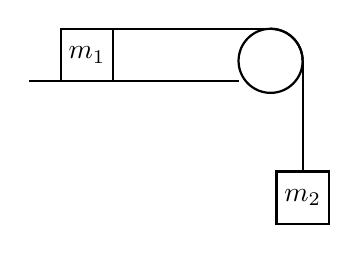
\begin{tikzpicture}[scale=0.74]
  \draw[thick] (-3.0,1.00)--(0.60,1.00);
  \draw[thick] (-2.45,1.00) rectangle (-1.55,1.90);
  \node at (-2.00,1.45) {$m_1$};
  \draw[thick] (-1.55,1.90)--(1.15,1.90);
  \draw[thick] (1.15,1.90) arc[start angle=90,end angle=0,radius=0.55];
  \draw[thick] (1.70,1.35)--(1.70,-0.55);
  \draw[thick] (1.15,1.35) circle (0.55);
  \draw[thick] (1.25,-1.45) rectangle (2.15,-0.55);
  \node at (1.70,-1.00) {$m_2$};
\end{tikzpicture}
\end{minipage}\end{center}
\diagcaption{图 2.10}{水平物块与悬挂物通过定滑轮相连。}
\end{origexamplebox}

\begin{xesolution}
轻绳不可伸长，因此 $m_1$ 向右和 $m_2$ 向下的加速度大小相等，记为 $a$。无摩擦定滑轮与轻绳使绳两端张力均为 $T$，如解图所示：
\soldiagTwoTen
分别对两物体沿运动方向列牛顿第二定律：
\[
  T=m_1a,
  \qquad
  m_2g-T=m_2a.
\]
相加消去 $T$，得
\[
  \boxed{a=\frac{m_2g}{m_1+m_2}}.
\]
所以 $m_1$ 向右、$m_2$ 向下，加速度大小均为上式。绳张力为
\[
  T=m_1a=\frac{m_1m_2g}{m_1+m_2}.
\]
\end{xesolution}
